\documentclass{article}
\usepackage[margin=1in]{geometry}
\usepackage{array}
\usepackage{amsmath}
\usepackage{amssymb}
\usepackage{booktabs}
\usepackage{tikz}
\usepackage{float}
\usetikzlibrary{arrows.meta,positioning,calc,shapes.geometric}

\InputIfFileExists{ps7-header.tex}{}{
    \newcommand{\TeamName}{Team name here}
    \newcommand{\MemberOne}{Member 1 name here}
    \newcommand{\MemberOneCode}{Member 1 code here}
    \newcommand{\MemberTwo}{Member 2 name here}
    \newcommand{\MemberTwoCode}{Member 2 code here}
    \newcommand{\MemberThree}{Member 3 name here}
    \newcommand{\MemberThreeCode}{Member 3 code here}
    \newcommand{\MemberFour}{Member 4 name here}
    \newcommand{\MemberFourCode}{Member 4 code here}
}

\begin{document}

\begin{center}
\section*{Problem Session 7: Processor Design}
\textbf{CPE223 Computer Architecture}\\
\textbf{Team: \TeamName}\\
\textit{\MemberOne\ (\MemberOneCode)}\\
\textit{\MemberTwo\ (\MemberTwoCode)}\\
\textit{\MemberThree\ (\MemberThreeCode)}\\
\textit{\MemberFour\ (\MemberFourCode)}\\
\textbf{Deadline: 10 March 2026, 23:59}
\end{center}

\section*{1. Processor Model and Assumptions}
We use a single-bus processor model with registers \texttt{PC}, \texttt{IR}, \texttt{MAR}, \texttt{MDR}, \texttt{Y}, \texttt{Z}, and a general register \texttt{Rn}. The ALU takes inputs from \texttt{Y} and the bus, and latches results into \texttt{Z}. Memory transactions use \texttt{MAR/MDR}. The branch condition uses the Zero flag \(Z_f\) from the status register.

\subsection*{Micro-operation notation}
We use standard hardwired-control notation:
\begin{itemize}
    \item \texttt{Xout}: drive register \texttt{X} onto bus.
    \item \texttt{Xin}: latch bus value into \texttt{X}.
    \item \texttt{Read}, \texttt{Write}: memory read/write command.
    \item \texttt{Add}: ALU operation with inputs \(Y\) and bus.
\end{itemize}

\subsection*{Common instruction fetch for all instructions}
\begin{align*}
T_0 &: \; PC_{out},\; MAR_{in} \\
T_1 &: \; Read,\; MDR_{in},\; PC \leftarrow PC + 1 \\
T_2 &: \; MDR_{out},\; IR_{in}\; (\text{decode})
\end{align*}

\begin{figure}[H]
\centering
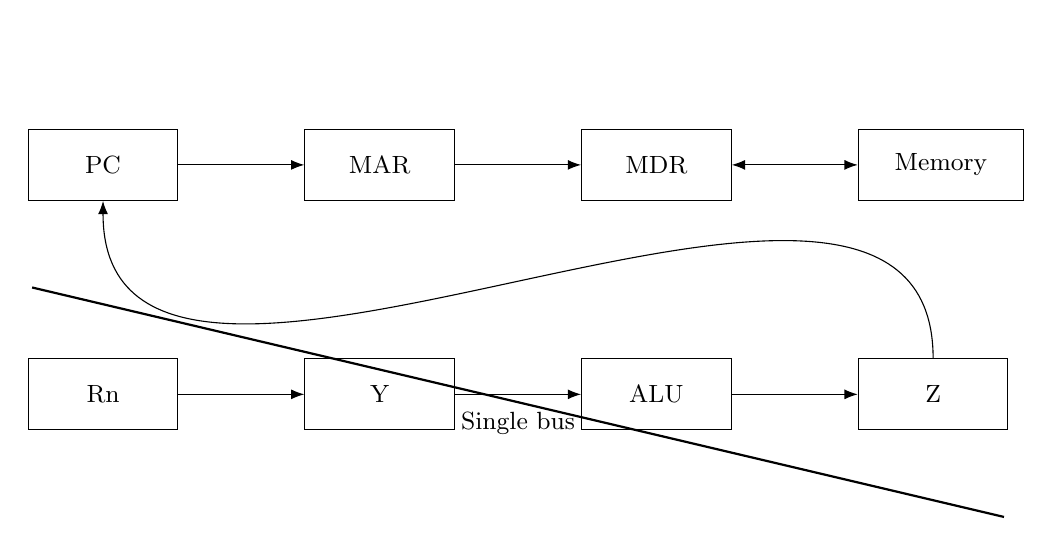
\begin{tikzpicture}[node distance=1.2cm and 1.6cm, >=Latex, every node/.style={font=\small}]
\node[draw, minimum width=1.9cm, minimum height=0.9cm] (pc) {PC};
\node[draw, minimum width=1.9cm, minimum height=0.9cm, right=of pc] (mar) {MAR};
\node[draw, minimum width=1.9cm, minimum height=0.9cm, right=of mar] (mdr) {MDR};
\node[draw, minimum width=2.1cm, minimum height=0.9cm, right=of mdr] (mem) {Memory};

\node[draw, minimum width=1.9cm, minimum height=0.9cm, below=2.0cm of pc] (rn) {Rn};
\node[draw, minimum width=1.9cm, minimum height=0.9cm, right=of rn] (y) {Y};
\node[draw, minimum width=1.9cm, minimum height=0.9cm, right=of y] (alu) {ALU};
\node[draw, minimum width=1.9cm, minimum height=0.9cm, right=of alu] (z) {Z};

\draw[thick] ($(pc.south)+(-0.9,-1.1)$) -- ($(z.south)+(0.9,-1.1)$) node[midway, below] {Single bus};

\draw[->] (pc) -- (mar);
\draw[->] (mar) -- (mdr);
\draw[<->] (mdr) -- (mem);
\draw[->] (rn) -- (y);
\draw[->] (y) -- (alu);
\draw[->] (alu) -- (z);
\draw[->] (z.north) to[out=90,in=-90] (pc.south);
\end{tikzpicture}
\caption{Baseline single-bus architecture used in this report.}
\end{figure}

\section*{2. Task 1: Stages and Data Paths (8 Instructions)}

\subsection*{2.1 ADD family}

\subsubsection*{(1) ADD Rn, off(Rn)}
Meaning: \(Rn \leftarrow Rn + M[Rn + off]\).
\begin{align*}
T_3 &: \; Rn_{out},\; Y_{in} \\
T_4 &: \; IR(off)_{out},\; Add,\; Z_{in} \quad (EA = Rn + off) \\
T_5 &: \; Z_{out},\; MAR_{in} \\
T_6 &: \; Read,\; MDR_{in} \\
T_7 &: \; Rn_{out},\; Y_{in} \\
T_8 &: \; MDR_{out},\; Add,\; Z_{in} \\
T_9 &: \; Z_{out},\; Rn_{in}
\end{align*}
Stage count: 10 total (\(T_0\) to \(T_9\)).

\subsubsection*{(2) ADD Rn, \#value}
Meaning: \(Rn \leftarrow Rn + imm\).
\begin{align*}
T_3 &: \; Rn_{out},\; Y_{in} \\
T_4 &: \; IR(imm)_{out},\; Add,\; Z_{in} \\
T_5 &: \; Z_{out},\; Rn_{in}
\end{align*}
Stage count: 6 total.

\subsubsection*{(3) ADD Rn, Rn}
Meaning: \(Rn \leftarrow Rn + Rn = 2Rn\).
\begin{align*}
T_3 &: \; Rn_{out},\; Y_{in} \\
T_4 &: \; Rn_{out},\; Add,\; Z_{in} \\
T_5 &: \; Z_{out},\; Rn_{in}
\end{align*}
Stage count: 6 total.

\begin{figure}[H]
\centering
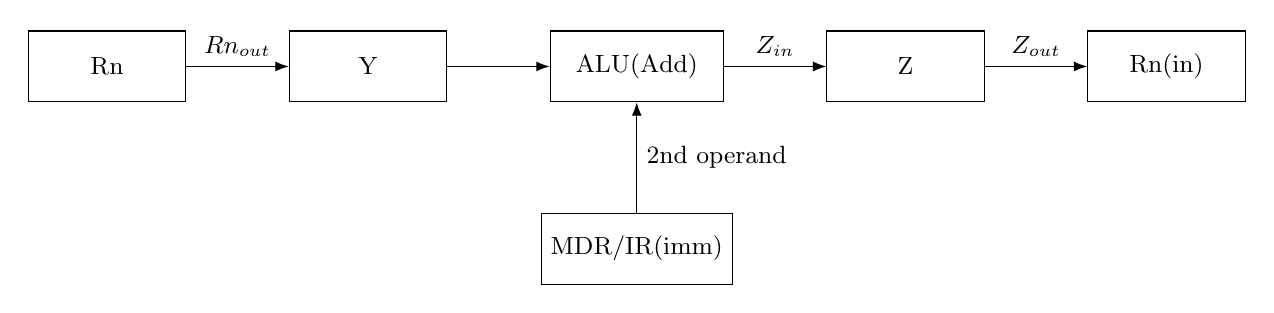
\begin{tikzpicture}[node distance=1.4cm and 1.3cm, >=Latex, every node/.style={font=\small}]
\node[draw, minimum width=2.0cm, minimum height=0.9cm] (rn) {Rn};
\node[draw, minimum width=2.0cm, minimum height=0.9cm, right=of rn] (y) {Y};
\node[draw, minimum width=2.2cm, minimum height=0.9cm, right=of y] (alu) {ALU(Add)};
\node[draw, minimum width=2.0cm, minimum height=0.9cm, right=of alu] (z) {Z};
\node[draw, minimum width=2.0cm, minimum height=0.9cm, right=of z] (rn2) {Rn(in)};
\node[draw, minimum width=2.0cm, minimum height=0.9cm, below=of alu] (mdr) {MDR/IR(imm)};

\draw[->] (rn) -- node[above]{\(Rn_{out}\)} (y);
\draw[->] (y) -- (alu);
\draw[->] (mdr) -- node[right]{2nd operand} (alu);
\draw[->] (alu) -- node[above]{\(Z_{in}\)} (z);
\draw[->] (z) -- node[above]{\(Z_{out}\)} (rn2);
\end{tikzpicture}
\caption{ADD-family execution flow. Second operand comes from \texttt{IR(imm)}, \texttt{Rn}, or \texttt{MDR}.}
\end{figure}

\subsection*{2.2 MOV family}

\subsubsection*{(4) MOV Rn, (Rn)}
Meaning: \(Rn \leftarrow M[Rn]\).
\begin{align*}
T_3 &: \; Rn_{out},\; MAR_{in} \\
T_4 &: \; Read,\; MDR_{in} \\
T_5 &: \; MDR_{out},\; Rn_{in}
\end{align*}
Stage count: 6 total.

\subsubsection*{(5) MOV (index), Rn}
Meaning: \(M[index] \leftarrow Rn\).
\begin{align*}
T_3 &: \; IR(index)_{out},\; MAR_{in} \\
T_4 &: \; Rn_{out},\; MDR_{in} \\
T_5 &: \; Write\quad (M[MAR] \leftarrow MDR)
\end{align*}
Stage count: 6 total.

\begin{figure}[H]
\centering
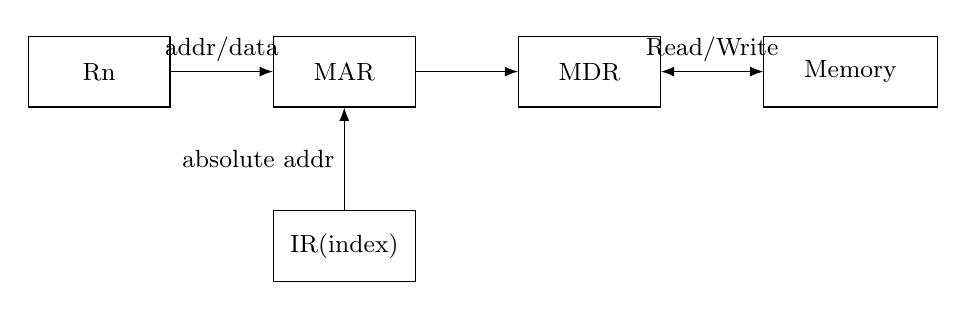
\begin{tikzpicture}[node distance=1.3cm and 1.3cm, >=Latex, every node/.style={font=\small}]
\node[draw, minimum width=1.8cm, minimum height=0.9cm] (rn) {Rn};
\node[draw, minimum width=1.8cm, minimum height=0.9cm, right=of rn] (mar) {MAR};
\node[draw, minimum width=1.8cm, minimum height=0.9cm, right=of mar] (mdr) {MDR};
\node[draw, minimum width=2.2cm, minimum height=0.9cm, right=of mdr] (mem) {Memory};
\node[draw, minimum width=1.8cm, minimum height=0.9cm, below=of mar] (ir) {IR(index)};

\draw[->] (rn) -- node[above]{addr/data} (mar);
\draw[->] (mar) -- (mdr);
\draw[<->] (mdr) -- node[above]{Read/Write} (mem);
\draw[->] (ir) -- node[left]{absolute addr} (mar);
\end{tikzpicture}
\caption{MOV-family data paths for load \texttt{MOV Rn,(Rn)} and store \texttt{MOV(index),Rn}.}
\end{figure}

\subsection*{2.3 Branch family}

\subsubsection*{(6) BZ (Rn)}
Meaning: if \(Z_f=1\), branch indirect through memory: \(PC \leftarrow M[Rn]\).
\begin{align*}
T_3 &: \; \text{if } Z_f=0 \text{ then End};\; \text{if } Z_f=1: Rn_{out},\; MAR_{in} \\
T_4 &: \; Read,\; MDR_{in} \\
T_5 &: \; MDR_{out},\; PC_{in}
\end{align*}
Stage count: 4 stages when not taken (ends at \(T_3\)); 6 stages when taken.

\subsubsection*{(7) BZ +\#relative}
Meaning: if \(Z_f=1\), \(PC \leftarrow PC + rel\).
\begin{align*}
T_3 &: \; \text{if } Z_f=0 \text{ then End};\; \text{if } Z_f=1: PC_{out},\; Y_{in} \\
T_4 &: \; IR(rel)_{out},\; Add,\; Z_{in} \\
T_5 &: \; Z_{out},\; PC_{in}
\end{align*}
Stage count: 4 stages when not taken; 6 stages when taken.

\subsubsection*{(8) B \#Absolute}
Meaning: unconditional branch \(PC \leftarrow abs\).
\begin{align*}
T_3 &: \; IR(abs)_{out},\; PC_{in}
\end{align*}
Stage count: 4 total.

\begin{figure}[H]
\centering
\begin{tikzpicture}[node distance=1.2cm and 1.5cm, >=Latex, every node/.style={font=\small}]
\node[draw, diamond, aspect=2.0, minimum width=2.4cm, minimum height=1.0cm] (zf) {\(Z_f=1?\)};
\node[draw, minimum width=2.0cm, minimum height=0.9cm, below left=1.3cm and 1.8cm of zf] (fetch) {Next fetch};
\node[draw, minimum width=2.1cm, minimum height=0.9cm, below right=1.3cm and 1.8cm of zf] (target) {Target path};
\node[draw, minimum width=2.0cm, minimum height=0.9cm, below=of target] (pc) {PC in};

\draw[->] (zf) -- node[above left]{No} (fetch);
\draw[->] (zf) -- node[above right]{Yes} (target);
\draw[->] (target) -- node[right]{abs / rel / mem[Rn]} (pc);
\end{tikzpicture}
\caption{Branch-family control flow. \texttt{BZ} is gated by \(Z_f\); \texttt{B\#Absolute} bypasses the condition.}
\end{figure}

\section*{3. Task 2: Hardwired Control (Yin, Zin, Rnin, MARin)}
This section covers the required instruction subset:
\texttt{ADD Rn,off(Rn)}, \texttt{ADD Rn,\#value}, \texttt{ADD Rn,Rn}, \texttt{BZ(Rn)}.

\subsection*{3.1 Instruction-class encoding}
\begin{align*}
I_{AO} &: \text{ADD Rn,off(Rn)} \\
I_{AI} &: \text{ADD Rn,\#value} \\
I_{AR} &: \text{ADD Rn,Rn} \\
I_{BZ} &: \text{BZ(Rn)}
\end{align*}
\(T_k\) denotes one-hot timing state \(k\), and \(Z_f\) is the branch condition flag.

\subsection*{3.2 Control-step table for required signals}
\begin{table}[H]
\centering
\renewcommand{\arraystretch}{1.25}
\begin{tabular}{@{}llcccc@{}}
\toprule
Instruction & Active step & Yin & Zin & Rnin & MARin \\
\midrule
Any of 4 instructions & \(T_0\) (fetch) & 0 & 0 & 0 & 1 \\
\midrule
\(I_{AO}\) & \(T_3\) & 1 & 0 & 0 & 0 \\
\(I_{AO}\) & \(T_4\) & 0 & 1 & 0 & 0 \\
\(I_{AO}\) & \(T_5\) & 0 & 0 & 0 & 1 \\
\(I_{AO}\) & \(T_7\) & 1 & 0 & 0 & 0 \\
\(I_{AO}\) & \(T_8\) & 0 & 1 & 0 & 0 \\
\(I_{AO}\) & \(T_9\) & 0 & 0 & 1 & 0 \\
\midrule
\(I_{AI}\) & \(T_3\) & 1 & 0 & 0 & 0 \\
\(I_{AI}\) & \(T_4\) & 0 & 1 & 0 & 0 \\
\(I_{AI}\) & \(T_5\) & 0 & 0 & 1 & 0 \\
\midrule
\(I_{AR}\) & \(T_3\) & 1 & 0 & 0 & 0 \\
\(I_{AR}\) & \(T_4\) & 0 & 1 & 0 & 0 \\
\(I_{AR}\) & \(T_5\) & 0 & 0 & 1 & 0 \\
\midrule
\(I_{BZ}\) taken path & \(T_3\) & 0 & 0 & 0 & \(Z_f\) \\
\bottomrule
\end{tabular}
\caption{Hardwired control activity for the requested four output signals.}
\end{table}

\subsection*{3.3 Boolean equations (sum-of-products)}
Define \(I_4 = I_{AO} + I_{AI} + I_{AR} + I_{BZ}\). Then:
\begin{align*}
Y_{in} &= T_3(I_{AO}+I_{AI}+I_{AR}) + T_7 I_{AO} \\
Z_{in} &= T_4(I_{AO}+I_{AI}+I_{AR}) + T_8 I_{AO} \\
Rn_{in} &= T_9 I_{AO} + T_5(I_{AI}+I_{AR}) \\
MAR_{in} &= T_0 I_4 + T_5 I_{AO} + T_3 I_{BZ} Z_f
\end{align*}

\subsection*{3.4 Branch-condition gating for \texttt{BZ(Rn)}}
The branch-indirect memory access is enabled only when \(Z_f=1\). Therefore, \(MAR_{in}\) at \(T_3\) is multiplied by \(Z_f\): when \(Z_f=0\), the execute phase terminates and control returns directly to fetch of the next sequential instruction.

\begin{figure}[H]
\centering
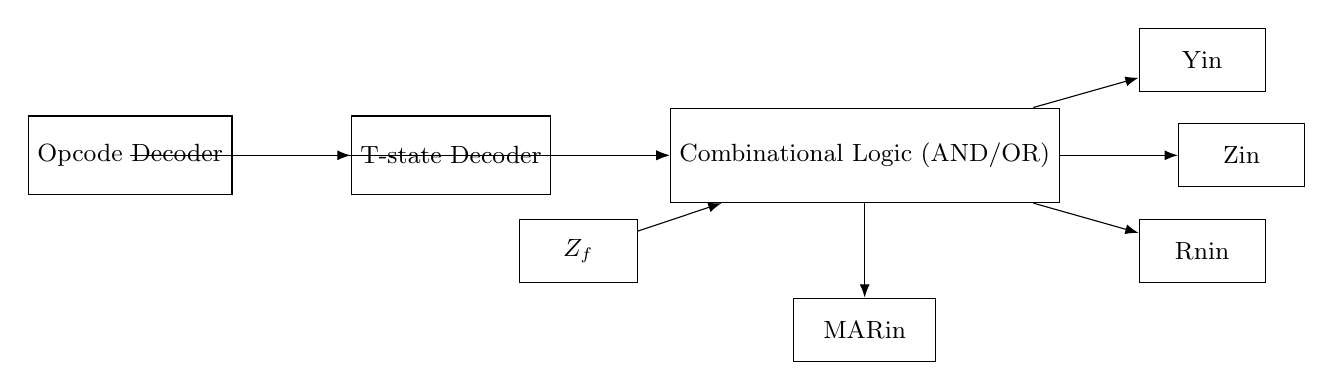
\begin{tikzpicture}[node distance=1.2cm and 1.5cm, >=Latex, every node/.style={font=\small}]
\node[draw, minimum width=2.4cm, minimum height=1.0cm] (op) {Opcode Decoder};
\node[draw, minimum width=2.4cm, minimum height=1.0cm, right=of op] (ts) {T-state Decoder};
\node[draw, minimum width=3.3cm, minimum height=1.2cm, right=of ts] (comb) {Combinational Logic (AND/OR)};
\node[draw, minimum width=1.6cm, minimum height=0.8cm, above right=0.2cm and 1.0cm of comb] (yin) {Yin};
\node[draw, minimum width=1.6cm, minimum height=0.8cm, right=of comb] (zin) {Zin};
\node[draw, minimum width=1.6cm, minimum height=0.8cm, below right=0.2cm and 1.0cm of comb] (rnin) {Rnin};
\node[draw, minimum width=1.8cm, minimum height=0.8cm, below=of comb] (marin) {MARin};
\node[draw, minimum width=1.5cm, minimum height=0.8cm, below left=0.2cm and 0.4cm of comb] (zf) {\(Z_f\)};

\draw[->] (op) -- (ts);
\draw[->] (ts) -- (comb);
\draw[->] (op) |- (comb);
\draw[->] (zf) -- (comb);
\draw[->] (comb) -- (yin);
\draw[->] (comb) -- (zin);
\draw[->] (comb) -- (rnin);
\draw[->] (comb) -- (marin);
\end{tikzpicture}
\caption{Hardwired control generation for \texttt{Yin, Zin, Rnin, MARin}.}
\end{figure}

\section*{4. Discussion: Stage Count and Data-Path Complexity}
\begin{table}[H]
\centering
\renewcommand{\arraystretch}{1.25}
\begin{tabular}{@{}lll@{}}
\toprule
Instruction & Total stages & Main complexity driver \\
\midrule
\texttt{ADD Rn,off(Rn)} & 10 & Effective address + memory read + ALU update \\
\texttt{ADD Rn,\#value} & 6 & One ALU operation with immediate \\
\texttt{ADD Rn,Rn} & 6 & One ALU operation with register operand \\
\texttt{MOV Rn,(Rn)} & 6 & Indirect memory read \\
\texttt{MOV(index),Rn} & 6 & Absolute address + memory write \\
\texttt{BZ(Rn)} & 4/6 & Conditional gating + indirect target fetch \\
\texttt{BZ +\#relative} & 4/6 & Conditional gating + PC-relative ALU add \\
\texttt{B \#Absolute} & 4 & Direct PC load \\
\bottomrule
\end{tabular}
\caption{Instruction complexity comparison in the single-bus processor.}
\end{table}

Immediate and register instructions are shorter because they avoid additional memory target fetches. Memory-indirect and branch-indirect forms require extra address generation and memory cycles, which increase both stage count and control complexity. In a single-bus design, each extra data transfer usually consumes another clock state, so addressing mode complexity directly dominates execution length and hardwired-control logic size.

\section*{5. Conclusion}
This report provides complete stage and data-path designs for all 8 required instructions and a hardwired-control derivation for \texttt{Yin}, \texttt{Zin}, \texttt{Rnin}, and \texttt{MARin} on the required 4-instruction subset. The analysis shows that in a single-bus architecture, addressing mode choice strongly determines both the number of execution stages and control-circuit complexity.

\end{document}
